\subsection{Data From \gls{smc}}
In \cref{sec:queries} we discussed different queries relevant for collecting data from the schedule, here we will illustrate what this data may look like, and discuss the usefulness thereof. We will in particular focus on the queries with keyword \textit{simulate}, as they are there for the purpose of extracting data.

First consider \cref{eq:smc4}, this query will result in a graph showing what payloads was supposed to run when and whether or not they were so. We have run this query through the UPPAAL GUI and resulting the graph seen in \cref{fig:active_running}. It should be noted that such graphs are not made available to the user via our system, but all the values needed to make such a graph is saved and made available to the user.

\begin{figure}[!h]
	\centering
	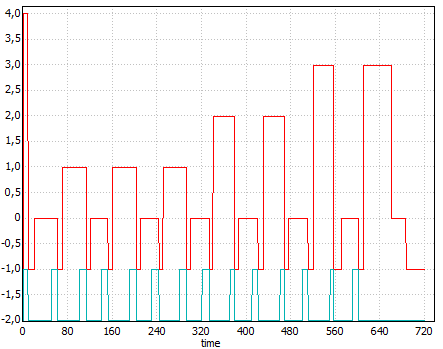
\includegraphics[scale=0.8]{graphics/active_running.png}
	\caption{Result of running query \ref{eq:smc4} in the UPPAAL GUI}
	\label{fig:active_running}
\end{figure}

We can in \cref{fig:active_running} see that all payloads are executed except for the last two. This can be seen by looking at the parts where the red curve is different from $-1$, if the blue curve at any time in this period differs from $-2$ it means the payload was executed. \\
The reason for the last two not being executed, is that executing them would result in depletion of the available well, as can be seen in \cref{fig:simAB}. 

\begin{figure}[!h]
	\centering
	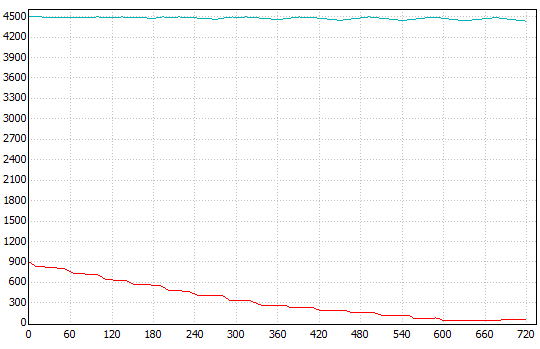
\includegraphics[scale=0.8]{graphics/simAB1.png}
	\caption{Result of running query \ref{eq:smc5} in the UPPAAL GUI}
	\label{fig:simAB}
\end{figure}
\ofx{talk about the above graph}